\documentclass[12pt]{article}

\usepackage{hcmus-report-template}

% Disable indentation on new paragraphs
\setlength{\parindent}{0pt}

% Line spacing 1.5
\renewcommand{\baselinestretch}{1.3}

% Optional: graphic path
% \graphicspath{PATH_TO_GRAPHIC_FOLDER}

% To use Times font family, uncomment this row
% \usepackage{mathptmx}

% To use roman section / subsection, uncomment these rows
% \renewcommand{\thesection}{\Roman{section}}
% \renewcommand{\thesubsection}{\thesection.\Roman{subsection}}

% Define course name, report name and report title.
\newcommand{\coursename}{Pattern Recognition}
\newcommand{\reportname}{Pattern Recognition Innovations}
\newcommand{\reporttitle}{Report Individual Exercise 1}

\newcommand{\studentname}{Le Truong Thinh (23127018)}
\newcommand{\teachername}{Vo Thanh Lam\\Nguyen Thanh Tinh}

% Header
\lhead{\reporttitle}
\rhead{
University of Science - VNU HCMC\\
\coursename
}

% Footer
% \newcommand{\leftfooter}{\LaTeX\ by \href{https://github.com/trhgquan}{Quan, Tran Hoang}}
% \lfoot{\leftfooter}

\newtheorem{definition}{Definition}
\newtheorem{theorem}{Theorem}
\newtheorem{lemma}{Lemma}


% ============ DOCUMENT ============
\begin{document}

\pagenumbering{roman}
\input{content/title.tex}

\tableofcontents
\pagebreak
% \listoftables
% \pagebreak
% \listoffigures
% \pagebreak

\pagenumbering{arabic}
\setcounter{page}{1}

\section{Tiêu đề \& Thành viên}

\subsection{Tên đồ án}
\textbf{Phân tích động lực thị trường và giá/thanh lý của ETH, meme coin (DOGE), alt-coin (SOL,...) trong giai đoạn quý 1 2024 (tháng 1/2024 - 3/2024)}

\subsection{Danh sách thành viên}
\begin{enumerate}
    \item Lê Trường Thịnh - 23127018
    \item Nguyễn Hoàng Anh Khoa - 23127015
    \item Lê Quốc Anh - 23127150
    \item Trần Tuấn Kiệt - 23127215
    \item Vũ Thành Đạt - 23127346
\end{enumerate}

\subsection{Bảng phân công công việc}
\begin{table}[H]
\centering
\begin{tabular}{|c|l|l|c|}
\hline
\textbf{STT} & \textbf{Họ và tên} & \textbf{Công việc cụ thể} & \textbf{Đóng góp} \\ \hline
1 & Lê Trường Thịnh & Thu thập dữ liệu & 100\% \\ \hline
2 & Nguyễn Hoàng Anh Khoa & Tiền xử lý dữ liệu & 100\% \\ \hline
3 & Lê Quốc Anh & Thiết kế trực quan hóa & 100\% \\ \hline
4 & Trần Tuấn Kiệt & Triển khai code trực quan & 100\% \\ \hline
5 & Vũ Thành Đạt & Viết báo cáo \& Phân tích & 100\% \\ \hline
\end{tabular}
\caption{Bảng phân công công việc thành viên nhóm}
\end{table}

\section{Giới thiệu Dữ liệu}

\subsection{Nguồn gốc dữ liệu}
Dữ liệu được thu thập từ sàn giao dịch tiền điện tử \textbf{Binance} thông qua nền tảng \textbf{Binance Vision} \cite{binancevision_futures_data}. Đây là nguồn dữ liệu chính thống cho phép truy cập vào dữ liệu lịch sử của thị trường tương lai (Futures) với độ chi tiết cao.

\textbf{Link tải dữ liệu:} \url{https://data.binance.vision/?prefix=data/futures/cm/daily/}

\subsection{Mô tả sơ lược}
Bộ dữ liệu tập trung vào các đồng tiền điện tử phổ biến như Ethereum (ETH), Dogecoin (DOGE), và Solana (SOL) trong giai đoạn quý 1 năm 2024. Dữ liệu bao gồm các thành phần chính sau:

\begin{itemize}
    \item \textbf{Dữ liệu nến giá (Klines):} Cung cấp thông tin OHLCV (Open, High, Low, Close, Volume) theo từng khung thời gian.
    \item \textbf{Dữ liệu lệnh thanh lý (Liquidations):} Thông tin chi tiết về các vị thế bị thanh lý trên thị trường.
    \item \textbf{Dữ liệu chỉ số phái sinh (Metrics):} Bao gồm tổng hợp đồng mở (Open Interest) và tỷ lệ Long/Short.
\end{itemize}

\subsection{Chi tiết các trường dữ liệu}

\subsubsection{Dữ liệu nến giá (Kline)}
\begin{table}[H]
\centering
\begin{tabular}{|l|l|l|}
\hline
\textbf{Tên trường} & \textbf{Kiểu dữ liệu} & \textbf{Mô tả} \\ \hline
open\_time & Long & Thời gian mở nến (Unix timestamp). \\ \hline
open, high, low, close & Float & Các mức giá trong phiên. \\ \hline
volume & Float & Khối lượng giao dịch. \\ \hline
close\_time & Long & Thời gian đóng nến. \\ \hline
base\_asset\_volume & Float & Khối lượng tính theo đồng coin cơ sở. \\ \hline
\end{tabular}
\end{table}

\subsubsection{Dữ liệu lệnh thanh lý}
\begin{table}[H]
\centering
\begin{tabular}{|l|l|l|}
\hline
\textbf{Tên trường} & \textbf{Kiểu dữ liệu} & \textbf{Mô tả} \\ \hline
time & Long & Thời gian xảy ra thanh lý. \\ \hline
side & String & Phía thanh lý (BUY/SELL). \\ \hline
price & Float & Giá tại thời điểm thanh lý. \\ \hline
original\_quantity & Float & Số lượng vị thế bị thanh lý. \\ \hline
\end{tabular}
\end{table}

\section{Các câu hỏi phân tích}
Nhóm đề xuất các câu hỏi phân tích sau:

\begin{itemize}
    \item \textbf{Câu hỏi 1:} Trong giai đoạn trên, xu hướng giá ETH biến động như thế nào so với các đường trung bình trượt giá đóng 7 cây nến?
    \item \textbf{Câu hỏi 2:} Mức độ tương quan giữa biến động giá của các coin diễn ra như thế nào trong các giai đoạn thị trường hưng phấn hoặc hoảng loạn?
    \item \textbf{Câu hỏi 3:} Tại các thời điểm xuất hiện "nến đỏ dài" (giá giảm mạnh trong thời gian ngắn), hợp đồng mở và khối lượng thanh lý thay đổi như thế nào? Có phải áp lực thanh lý lệnh "Long" là nguyên nhân chính dẫn đến đà giảm sâu?
    \item \textbf{Câu hỏi 4:} Khối lượng thanh lý, hợp đồng mở theo thời gian như thế nào trong một "ngày sập giá", theo dõi?
    \item \textbf{Câu hỏi 5:} Liệu có thể \textbf{dự đoán} các "trạng thái thị trường" hưng phấn, hoảng loạn (sập giá) dựa trên sự kết hợp giữa mất cân bằng thanh lý (khối lượng thanh lý lệnh Long $\gg$ Short hoặc ngược lại), tăng/giảm đột biến của hợp đồng mở, giá trong dữ liệu trên?
\end{itemize}

\section{Thiết kế \& Kết quả (The "How")}

\subsection{Screenshot toàn bộ Dashboard}
\begin{figure}[H]
    \centering
    % \includegraphics[width=\textwidth]{img/dashboard_full.png}
    \caption{Giao diện tổng quan của Dashboard}
\end{figure}

\subsection{Trình bày chi tiết \& Giải thích thiết kế}

\subsubsection{Biểu đồ Nến \& Khối lượng kết hợp Đường Trung bình (MA)}
\begin{figure}[H]
    \centering
    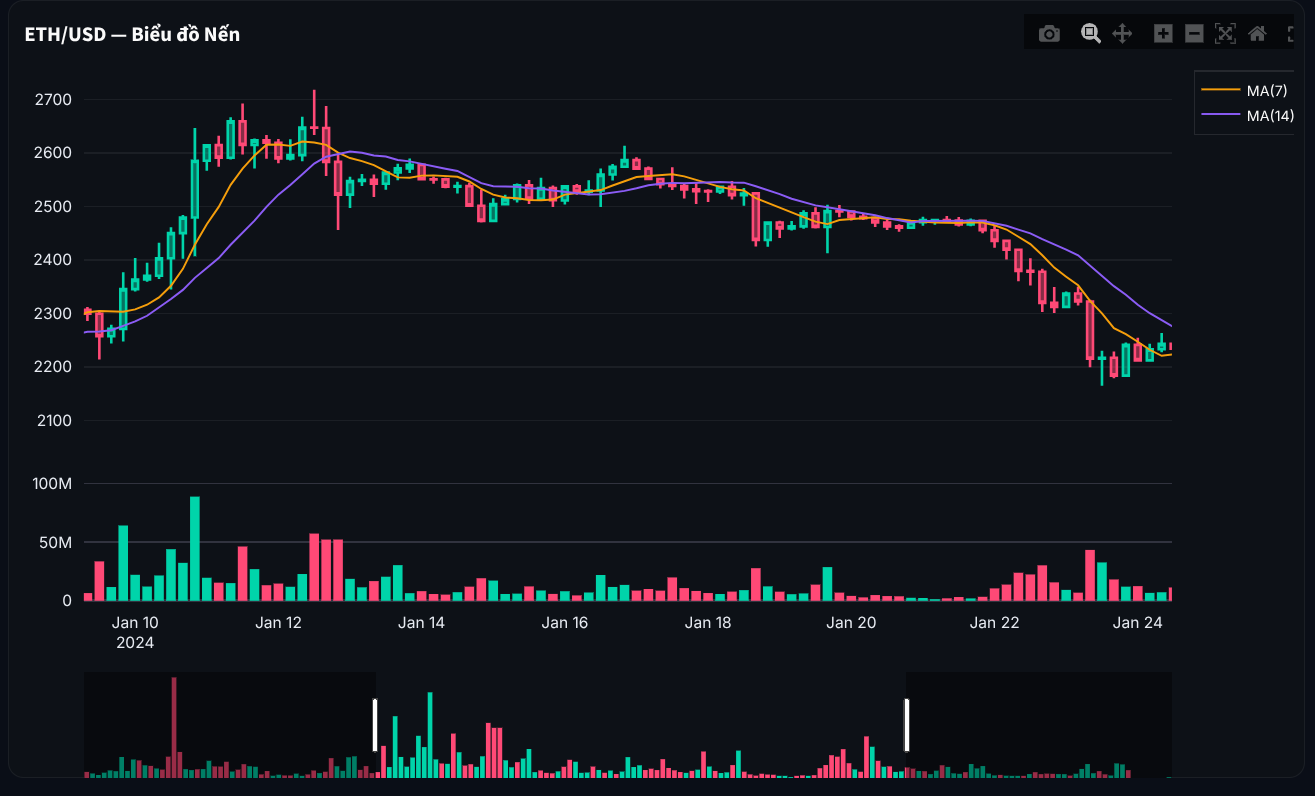
\includegraphics[width=\textwidth]{img/sol_candlestick.png}
    \caption{Biểu đồ nến SOL/USD cùng Khối lượng giao dịch và Đường Trung bình 7 \& 14}
\end{figure}

\textbf{Giải thích thiết kế (Marks \& Channels):}
Dựa trên lý thuyết Trực quan hóa dữ liệu, biểu đồ này sử dụng các Marks (Dấu hiệu) và Channels (Kênh hiển thị) như sau để mã hóa thông tin:

\begin{itemize}
    \item \textbf{Thành phần Nến giá (Candlestick):}
    \begin{itemize}
        \item \textbf{Mark:} Area/Shape (Hình chữ nhật thân nến - Open/Close) và Line (Đường thẳng bóng nến - High/Low).
        \item \textbf{Channel - Vị trí (Position):} Trục X là thời gian, Trục Y là mức giá.
        \item \textbf{Channel - Chiều dài (Size/Length):} Chiều dài thân nến thể hiện độ chênh lệch giữa giá mở cửa và đóng cửa, trong khi thân bóng nến biểu thị biên độ biến động giá trong phiên.
        \item \textbf{Channel - Màu sắc (Color):} Dùng để mã hóa tính chất thay đổi (Kênh Hue). Màu xanh (Identity/Category: Tăng) cho nến đóng cao hơn giá mở, và màu đỏ/hồng cho nến đóng thấp hơn giá mở.
    \end{itemize}
    
    \item \textbf{Thành phần Đường Trung bình động (Moving Average - MA7, MA14):}
    \begin{itemize}
        \item \textbf{Mark:} Line (Đường cong liên tục).
        \item \textbf{Channel - Vị trí (Position):} Trục Y thể hiện mức giá trung bình ứng trên trục X thời gian.
        \item \textbf{Channel - Màu sắc (Color):} Sử dụng màu Cam cho MA(7) và màu Tím cho MA(14). Mục đích cũng là kênh Hue dùng để Phân biệt (Identify) hai chuỗi dữ liệu đường trung bình khác nhau.
    \end{itemize}

    \item \textbf{Thành phần Khối lượng giao dịch (Volume Bar Chart dưới cùng):}
    \begin{itemize}
        \item \textbf{Mark:} Line/Bar (Cột dọc hẹp).
        \item \textbf{Channel - Vị trí (Position):} Đồng bộ trục X thời gian với nến giá phía trên, nhưng trục Y được đặt độc lập thấp bên dưới với thang đo riêng về khối lượng.
        \item \textbf{Channel - Chiều dài (Size/Length):} Chiều cao của cột trên trục Y thể hiện độ lớn định lượng Khối lượng giao dịch.
        \item \textbf{Channel - Màu sắc (Color):} Đồng bộ sắc độ với màu của nến trên cùng khung giờ (xanh hoặc đỏ) để người xem có thể đánh giá nhanh tương quan khối lượng với việc giá tăng/giảm.
    \end{itemize}
\end{itemize}

\textbf{Nhận xét (Insights):}
\begin{itemize}
    \item Xu hướng giá chung từ khoảng 24/Jan/2024 đến 30/Jan/2024 thể hiện đà phục hồi và tăng trưởng của đồng SOL. Đường MA(7) màu cam có xu hướng vượt lên trên đường MA(14) màu tím, xác nhận cấu trúc giao cắt đồng thuận với đà tăng giá ngắn hạn.
    \item Tại các cây nến đỏ sâu trước ngày 24/Jan, cột volume vượt trội cho thấy áp lực bán rát cao. Tuy nhiên, sau vùng giá tạo đáy (ngày 24/Jan), áp lực bán đã suy giảm và lực mua chiếm ưu thế thể hiện qua sự xuất hiện liên tục của các nến xanh thân lớn nhịp nhàng với đà dốc lên của đường MA ngắn hạn.
\end{itemize}

\input{content/section/05}

% References
\cleardoublepage
\phantomsection
\addcontentsline{toc}{section}{References}
\bibliographystyle{abbrvurl}
\bibliography{ref/ref}

% Appendix
\appendix
% Add \cleardoublepage to move appendices to next page.
% \section{Appendix}

\begin{figure}[H]
    \centering
    \includegraphics[width=0.8\textwidth]{img/arcfaceframework.png}
    \caption{ArcFace training framework}
\end{figure}


\begin{figure}[H]
\centering
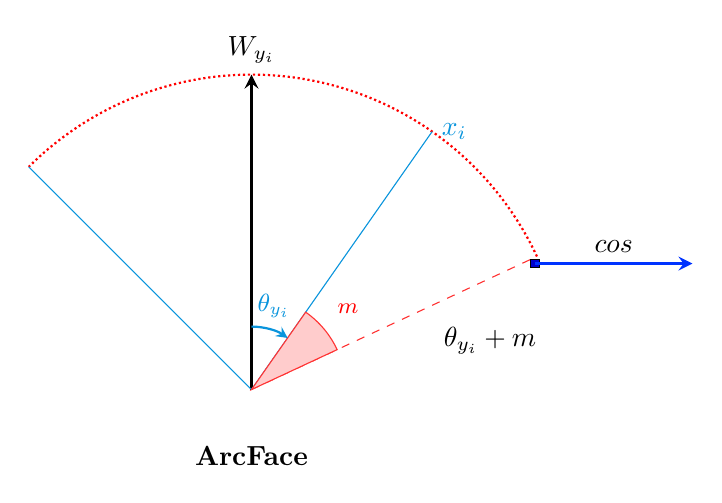
\begin{tikzpicture}[scale=2, >=stealth]
    % Origin
    \coordinate (O) at (0,0);
    \def\R{2} % Radius

    % --- W_yi Vector (Vertical) ---
    \draw[->, black, very thick] (O) -- (90:\R) node[above] {$W_{y_i}$};

    % --- Sector Arc (Red Dotted) ---
    % Spanning from roughly 135 to 25 degrees
    \draw[red, densely dotted, thick] (25:\R) arc (25:135:\R);

    % --- Left Radial Line (Blue) ---
    \draw[cyan!80!blue, thin] (O) -- (135:\R);

    % --- Right Radial Line (Blue) - representing x_i ---
    % Let's place x_i at 55 degrees (theta = 35)
    % And margin end at 25 degrees (m = 30)
    \def\angX{55}
    \def\angM{25}
    
    \draw[cyan!80!blue, thin] (O) -- (\angX:\R);
    \node[cyan!80!blue, right] at (\angX:\R) {$x_i$};
    
    % --- Red Dashed Line (Margin Boundary) ---
    \draw[red!80, dashed, thin] (O) -- (\angM:\R);
    
    % --- Margin Wedge (Red Filled) ---
    \draw[fill=red!20, draw=red!80] (O) -- (\angX:0.6) arc (\angX:\angM:0.6) -- cycle;
    \node[red, font=\footnotesize] at ({(\angX+\angM)/2}:0.8) {$m$};

    % --- Angle Theta_yi (Blue Arc) ---
    \draw[cyan!80!blue, thick, ->] (90:0.4) arc (90:\angX:0.4);
    \node[cyan!80!blue, font=\small] at (75:0.55) {$\theta_{y_i}$};


    % --- Label theta + m ---
    % Pointing to the dashed line area
    \node[right, black] at (15:1.2) {$\theta_{y_i} + m$};

    % --- Cosine Arrow on Right ---
    \coordinate (sq) at (1.8, 0.8);
    \node[draw, fill=blue!80!black, inner sep=1.5pt] (sq_node) at (sq) {};
    \draw[->, blue!80!cyan, very thick] (sq) -- ++(1.0, 0) node[midway, above, black] {$cos$};

    % --- Bottom Label ---
    \node[below, font=\bfseries] at (0,-0.3) {ArcFace};
\end{tikzpicture}
\caption{$x_i$ is embedding feature, $W_{y_i}$ is (sub-)center. Want: mininize distance of arc (geodesic distance) on hypersphere.}
\end{figure}

\begin{figure}[H]
    \centering
    \includegraphics[width=0.8\textwidth]{img/arcFacehiststartend.pdf}
    \caption{Target angle ($\theta$) distributions during ArcFace training}
\end{figure}

\begin{figure}[H]
    \centering
    \includegraphics[width=0.8\textwidth]{img/multicenter.png}
    \caption{Example of sub-classes after sub-center ArcFace}
\end{figure}

\begin{figure}[H]
    \centering
    \includegraphics[width=0.8\textwidth]{img/CASIAvariancedistribution2ECCV.pdf}
    \caption{Clean data isolation (dominant) after sub-center ArcFace}
\end{figure}


% \begin{figure}[H]
%     \centering
%     \includegraphics[width=0.8\textwidth]{img/IJBC.pdf}
%     \caption{ROC for test set IJB-C, trained with ResNet100 and dataset above}
% \end{figure}

\end{document}